% Latex template: mahmoud.s.fahmy@students.kasralainy.edu.eg
% For more details: https://www.sharelatex.com/learn/Beamer

\documentclass[aspectratio=1610]{beamer}					% Document class

\setbeamertemplate{footline}[text line]{%
  \parbox{\linewidth}{\vspace*{-8pt}A brief introduction to graphical models and deep methods in computational network biology \hfill\insertshortauthor\hfill\insertpagenumber}}
\setbeamertemplate{navigation symbols}{}

\usepackage[english]{babel}				% Set language
\usepackage[utf8x]{inputenc}			% Set encoding

\mode<presentation>						% Set options
{
  \usetheme{default}					% Set theme
  \usecolortheme{default} 				% Set colors
  \usefonttheme{default}  				% Set font theme
  \setbeamertemplate{caption}[numbered]	% Set caption to be numbered
}

% Uncomment this to have the outline at the beginning of each section highlighted.
%\AtBeginSection[]
%{
%  \begin{frame}{Outline}
%    \tableofcontents[currentsection]
%  \end{frame}
%}

\usepackage{graphicx}					% For including figures
\usepackage{booktabs}					% For table rules
\usepackage{hyperref}					% For cross-referencing
\usepackage[absolute,overlay]{textpos}
\usepackage{bm}

\title{A brief introduction to graphical models and deep methods in computational network biology}	% Presentation title
\author{Clayton W. Seitz}								% Presentation author
\date{\today}									% Today's date	

\begin{document}

% Title page
% This page includes the informations defined earlier including title, author/s, affiliation/s and the date
\begin{frame}
  \titlepage
\end{frame}

% Outline
% This page includes the outline (Table of content) of the presentation. All sections and subsections will appear in the outline by default.
\begin{frame}{Outline}
  \tableofcontents
\end{frame}

% The following is the most frequently used slide types in beamer
% The slide structure is as follows:
%
%\begin{frame}{<slide-title>}
%	<content>
%\end{frame}

\section{A few example networks in biology}

\begin{frame}{Computational network biology}

Emerging research field that encompasses theory and applications of \textcolor{red}{network models} to study complex interactions of cells, DNA, RNA, proteins, and metabolites\\
\vspace{0.2in}
Say we have a set of variables $\bm{X} = (x_{1},x_{2},...,x_{n})$ which might have some statistical dependence. $\bm{X}$ might be expression data, for example\\
\vspace{0.2in}
\begin{itemize}
\item Often we are handed a batch of empirical samples $\bm{X} = \{\bm{x_{1}},..,\bm{x_{p}}\}$
\item We want to learn about the generating distribution $P(\bm{x},t)$
\end{itemize}

\vspace{0.2in}
Joint effort between physics, computer science, and biology

\begin{textblock*}{3cm}(12.25cm,5.5cm)
\begin{figure}
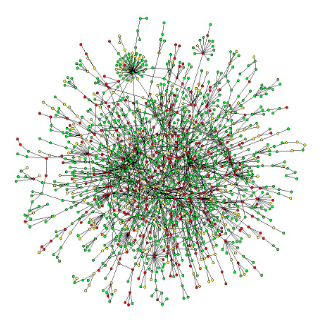
\includegraphics[width=3cm]{net.png}
\end{figure}
\end{textblock*}

\end{frame}

\begin{frame}{A gene interaction network}
\begin{center}
\begin{textblock*}{13cm}(1.3cm,1.5cm)
\begin{figure}
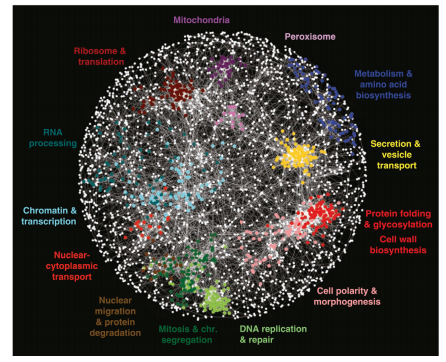
\includegraphics[width=8cm]{gene-network.png}
\caption{\textbf{Landscape of genetic interactions} in cells. Edges between genes denote Pearson correlation coefficients ($\rho > 0.2$) calculated from the
complete genetic interaction matrix.}
\end{figure}
\end{textblock*}
\end{center}
\end{frame}

\begin{frame}{A protein interaction network}
\begin{center}
\begin{textblock*}{13cm}(1.5cm,1cm)
\begin{figure}
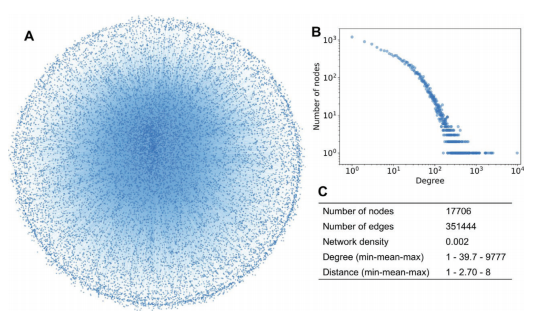
\includegraphics[width=10cm]{protein-interactome.png}
\caption{\textbf{Human protein interactome} of 17,706 proteins and 351,444 interactions (A) Overall complex network of human interactome. (B) Degree
(connectivity) distribution of proteins by following a power-law tail. (C) Several selected network topological characteristics of the interactome.}
\end{figure}
\end{textblock*}
\end{center}
\end{frame}

\begin{frame}{A cellular interaction network (model neurons)}
\begin{textblock*}{12cm}(0.5cm,0.75cm)
\begin{figure}
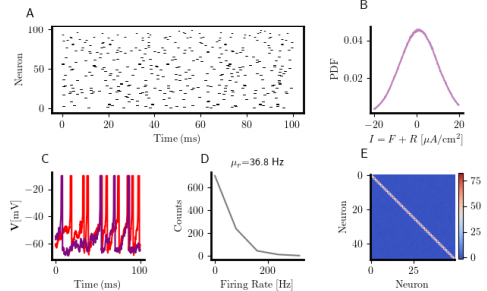
\includegraphics[width=11cm]{neural-network.png}
\caption{\textbf{Asychronous spiking of model neurons} (A) Steady-state raster plot of $N=100$ uncoupled EIF neurons undergoing stimulation with GWN with $\mu = 2\mu A/\mathrm{cm}^{2}$ and $\sigma = 9 \;\mu A/\mathrm{cm}^{2}$}
\end{figure}
\end{textblock*}
\begin{textblock*}{3cm}(12.25cm,0.5cm)
\begin{figure}
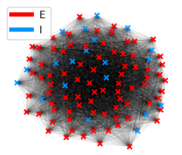
\includegraphics[width=3cm]{neural-network-graph.png}
\end{figure}
\end{textblock*}
\end{frame}

\section{Graphical models in a nutshell}
\begin{frame}{Probabilistic graphical models (PGMs)}

Probabilistic graphical models are a class of machine \\learning algorithms that represent statistical \\dependencies of probability distributions as graphs\\
\vspace{0.2in}
Two main types used in machine learning: \\\textcolor{red}{Bayesian Networks} (BNs), \textcolor{red}{Markov Random Fields} (MRFs), \\but there are others\\
\vspace{0.2in}
Major advantage is that they are \textcolor{red}{structured models}\\They do not scale as easily as deep networks


\begin{textblock*}{5cm}(10.75cm,1cm)
\begin{figure}
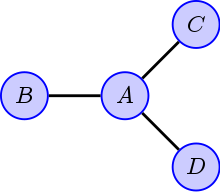
\includegraphics[width=4cm]{mrf.png}
\end{figure}
\end{textblock*}

\begin{textblock*}{5cm}(10.75cm,5cm)
\begin{figure}
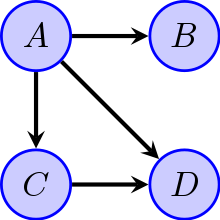
\includegraphics[width=2.75cm]{bayes-net.png}
\end{figure}
\end{textblock*}

\end{frame}


\begin{frame}{Probabilistic graphical models (PGMs)}

\begin{textblock*}{10cm}(1cm,1.5cm)
Say we have a joint probability over gene expression $P(\bm{X})$\\A PGM describes how $P(\bm{X})$ factors\\
\end{textblock*}

\begin{textblock*}{9cm}(1cm,3.5cm)
\textcolor{red}{Markov Random Fields} (MRFs) e.g., Ising model
\begin{equation*}
P(\bm{X};\Theta) = \frac{1}{Z}\prod_{\mathcal{C}} \psi_{\mathcal{C}}(x_{\mathcal{C}}; \Theta)
\end{equation*}
\end{textblock*}

\begin{textblock*}{7cm}(1cm,6.5cm)
\textcolor{red}{Bayesian Network} (BNs) - include causality
\begin{equation*}
P(\bm{X};\Theta) = \prod_{i=1}^{N}P(\bm{X_{i}}|pa(X_{i}),\Theta_{i})
\end{equation*}
\end{textblock*}


\begin{textblock*}{5cm}(10.75cm,1cm)
\begin{figure}
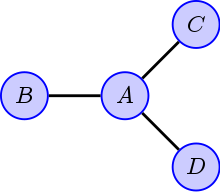
\includegraphics[width=4cm]{mrf.png}
\end{figure}
\end{textblock*}

\begin{textblock*}{5cm}(10.75cm,5cm)
\begin{figure}
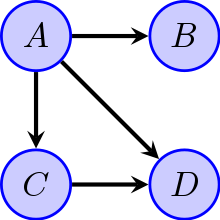
\includegraphics[width=2.75cm]{bayes-net.png}
\end{figure}
\end{textblock*}

\begin{textblock*}{15cm}(1cm,9cm)
BNs as well as hybrid models have been used to examine gene expression
\end{textblock*}

\end{frame}

\begin{frame}{An example Bayesian graphical model}

\begin{figure}
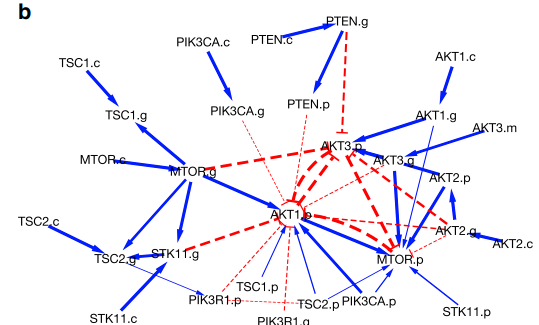
\includegraphics[width=11cm]{pi3k-pathway.png}
\caption{\textbf{PI3K pathway graph} discovery using graphical modeling (Ni et al. Bioinformatics 2018). c - transcript count, g - gene, p - protein, m - methylation}
\end{figure}
\end{frame}

\section{Issues with scaling graphical models and alternatives}
\begin{frame}{A tradeoff between mechanistic understanding and scale}

Fine structure of molecular interactions sometimes can be resolved for low dimensionality\\
\vspace{0.2in}
\textcolor{red}{Computational complexity} often scales exponentially with an increase in variables, density of interactions\\
\vspace{0.2in}
In high-dimensional biological networks we often turn to classic dimensionality reduction or deep methods\\
\vspace{0.2in}
Introducing \textcolor{red}{latent variables} into the model can reduce \\computational complexity


\begin{textblock*}{3cm}(12.25cm,5.5cm)
\begin{figure}
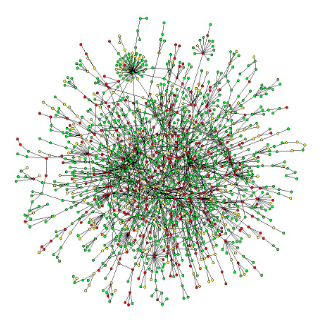
\includegraphics[width=3cm]{net.png}
\end{figure}
\end{textblock*}

\end{frame}

\begin{frame}{Latent variables}
Modeling all possible conditional dependencies quickly becomes intractable, lots of parameters\\
\vspace{0.2in}
Introducing latent variables $\bm{z}$ can reduce the number of needed parameters\\
\vspace{0.2in}

\begin{figure}
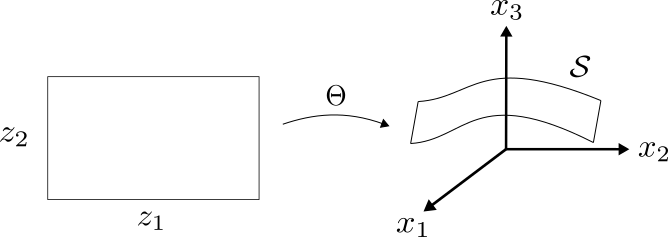
\includegraphics[width=0.8\textwidth]{manifold.png}
\end{figure}

\end{frame}


\begin{frame}{Variational autoencoders (VAEs)}
The VAE architecture has been very succesful when applied to RNA-seq datasets see (Lopez Nature Methods 2020)

\begin{center}
\begin{figure}
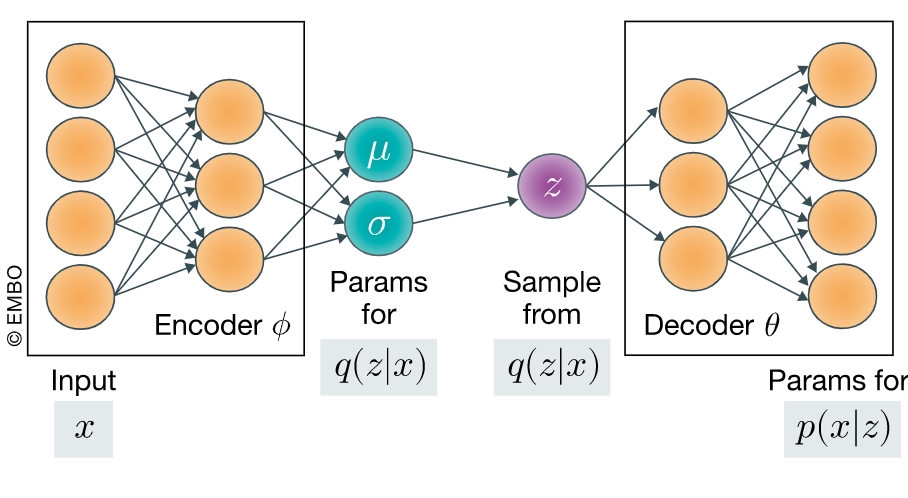
\includegraphics[width=0.8\textwidth]{vae}
\caption{\textbf{Variational autoencoder architecture} Lopez 2020 EMBO}
\end{figure}
\end{center}
\end{frame}

\begin{frame}{Using the VAE for cell phenotyping}

\begin{textblock*}{15cm}(0.75cm,1.5cm)
558 genes/3005 cells/7 cell types from mouse cortex - CORTEX\\
\vspace{0.1in}
7,397 genes/4016 cells/continuous for HEMATO - hematopoietic progenitor cells (see Lopez Nature Methods 2020)\\
\end{textblock*}
\begin{textblock*}{7cm}(0.75cm,3.5cm)
\begin{figure}
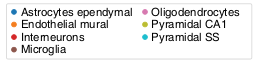
\includegraphics[width=7cm]{cortex-legend.png}
\end{figure}
\end{textblock*}
\begin{textblock*}{7cm}(0.75cm,5.5cm)
\begin{figure}
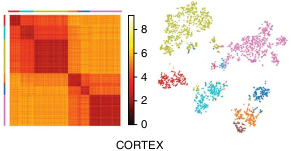
\includegraphics[width=7cm]{cortex.png}
\end{figure}
\end{textblock*}
\begin{textblock*}{7cm}(8.5cm,3.5cm)
\begin{figure}

\includegraphics[width=7cm]{hemato-legend.png}
\end{figure}
\end{textblock*}
\begin{textblock*}{7cm}(8.5cm,5.75cm)
\begin{figure}
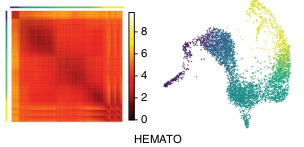
\includegraphics[width=7cm]{hemato.png}
\end{figure}
\end{textblock*}
\end{frame}

\section{References}

% Adding the option 'allowframebreaks' allows the contents of the slide to be expanded in more than one slide.
\begin{frame}[allowframebreaks]{References}
	\tiny\bibliography{references}
	\bibliographystyle{apalike}
\end{frame}

\end{document}